%%% Template originaly created by Karol Kozioł (mail@karol-koziol.net) and modified for ShareLaTeX use

\documentclass[a4paper,11pt]{amsart}


\usepackage{graphicx}
\usepackage{float}



\usepackage{geometry}
\geometry{total={210mm,297mm},
left=25mm,right=25mm,%
bindingoffset=0mm, top=20mm,bottom=20mm}

\linespread{1.3}

\newcommand{\linia}{\rule{\linewidth}{0.5pt}}
\newcommand\nobreakpar{\par\nobreak\@afterheading} 




% my own titles
\makeatletter
\renewcommand{\maketitle}{
\begin{center}
%\vspace{4ex}
{\huge{\@title}}
\vspace{1ex}
\\
\linia\\
%\@author \hfill \@date
\vspace{2ex}
\end{center}
}
\makeatother
%%%

% custom footers and headers
\usepackage{fancyhdr}
\pagestyle{fancy}
\chead{}
\rhead{\today}
\cfoot{}
\rfoot{Page \thepage}
\renewcommand{\headrulewidth}{0pt}
\renewcommand{\footrulewidth}{0pt}
%
\begin{document}
\author{By Group 7}

\title{Rules of the game}
    \vspace*{.6cm}

  {\let\newpage\relax\maketitle}
 


%%% BEGIN DOCUMENT

\section{Introduction}
\subsection{The Players}
Each player chooses one of six characters. No player may choose the same character as another player.
\begin{figure}[h]
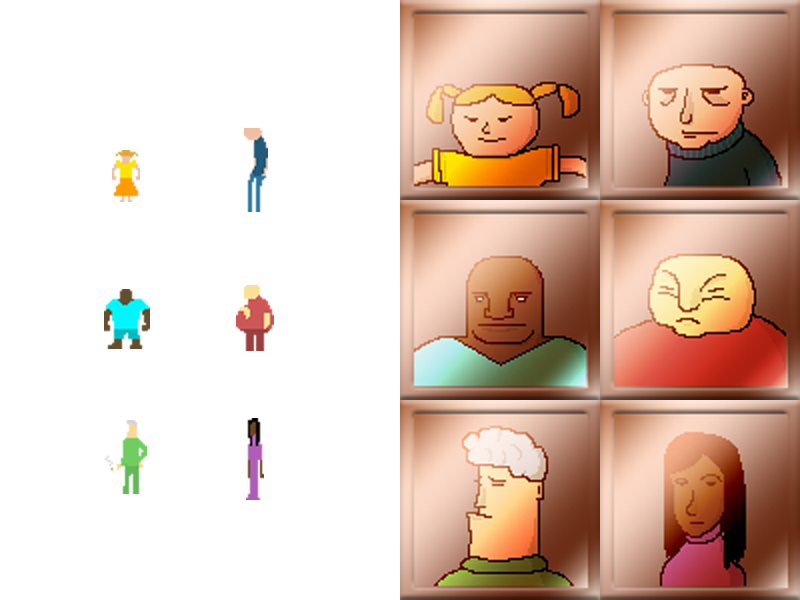
\includegraphics{characters}
\end{figure}

\subsection{The Goal}
Players compete for the position of President of the United States of America
\subsection{The Board}
Each side has ten fields a player can land on. 
\begin{figure}[H]
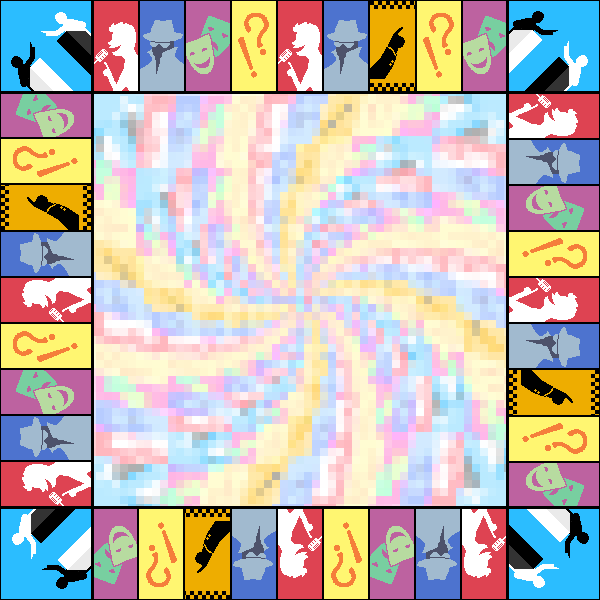
\includegraphics[width=\textwidth]{board}
\end{figure}
\subsection{The Cards}
After landing on an Action field, the player must draw a card from the top of the pile. The cards have the following effects: 
\begin{itemize}
\item Gain a Dirt card [8]
\item Lose Charisma [4]
\item Gain Charisma [6]
\item Move to player of choice [3]
\item Steal a Dirt card from player of choice [4]
\item Skip turn [2]
\item Make opponent skip turn [4]
\item Counter 1 Dirt card during a debate [6]
\item Trigger Debate with random opponent [4]
\item Trigger Debate with opponent of choice [2]
\item Delay the election by 10 turns [1]
\item Go to any field on the board [4]
\end{itemize} 

(The number of cards with that effect is listed in square brackets)

\section{Rules}
\subsection{How to move}
At the start of the game, players toss dice. The scores will dictate the order in which the player take turns. Player with the highest score goes first. In the event of a tie, the tie is resolved with another throw of the dice.

When a player starts a turn, two dice a thrown, and the player moves their character forward the same number of fields as the combined eyes of the tossed dice. The player must then perform an action as dictated by the field they landed on.
\subsection{Player attributes}
A player has two basic attributes: Charisma and Public Opinion. 
\subsection{Player Inventory}
Dirt cards are kept in the player's inventory.
\subsection{Fields on the board}
\subsubsection{Debate}Placed in each corner. Triggers a debate.
\subsubsection{Action}The player draws an action card.
\subsubsection{Informant}The player receives a dirt card on a player of choice.
\subsubsection{Taxi}The player moves back or forth 4 spaces.
\subsubsection{Acting Class}Player gets another point to charisma.

\section{Debates}
\subsection{Rules}
Each player of the debate has a "Debate Score", which will determine the outcome of the debate. The player with the highest Public Opinion score may add 1 point to their Debate Score.
\subsection{Tools for winning debates}
\subsubsection{Charisma}
A player's charisma is added to their Debate Score.
\subsubsection{Dirt}
Dirt on other players may be collected through action cards, or by landing on fields labeled "Informant". The player may choose how many dirt cards to play in the current debate. The points listed on the dirt cards are added to the Debate Score.
Only dirt on the debate opponent may be used, and cards are expended when used.

\subsection{Winning a debate}
Each player tosses a die. The number of eyes is added to the Debate Score. The player with the highest score wins. 20 percent of the loser's Public Opinion score is then subtracted from the loser and given to the winner.

\section{Winning the game}
\subsection{Turn 50}
When the last player has played 50 turns, the election is held. The player with the highest Public Opinion score wins. The score is first multiplied with the player's gerrymandering factor.
\end{document}








